
\newcommand{\base}{
    \def\radiusone{10mm}
    \def\radiustwo{5mm}
    \def\lengthone{1mm}
    \def\lengthtwo{0.5mm}
    \draw (\radiusone, -\lengthone - \lengthtwo) arc(0:-180:{\radiusone} and {0.5*\radiusone});
    \draw[yshift=-\lengthtwo] ellipse [x radius=\radiusone, y radius=0.5*\radiusone];
    \draw (-\radiusone, -\lengthone - \lengthtwo) -- (-\radiusone, -\lengthtwo);
    \draw (\radiusone, -\lengthone - \lengthtwo) -- (\radiusone, -\lengthtwo);
    \draw (\radiustwo, -\lengthtwo) arc(0:-180:{\radiustwo} and {0.5*\radiustwo});
    \draw ellipse [x radius=\radiustwo, y radius=0.5*\radiustwo];
    \draw (-\radiustwo, -\lengthtwo) -- (-\radiustwo, 0mm);
    \draw (\radiustwo, -\lengthtwo) -- (\radiustwo, 0mm);
}

\newcommand{\link}[1]{
    \draw circle [radius=0.5mm];
    \draw (#1) circle [radius=0.5mm];
    \draw [double distance=1mm, fill=white] (0,0) -- (#1);
}

% Draw an angle annotation
% Input:
%   #1 Angle offset (optional)
%   #2 Angle
%   #3 Label
% Example:
%   \angann[0.5]{30}{$\theta_1$}

\newcommand{\angann}[3][1]{%
    \def\ddx{#1cm}
    \begin{scope}[red]
    \draw [dashed, red] (0,0) -- (1.2*\ddx,0);
    \draw [->, shorten >=3.5pt] (\ddx,0) arc (0:#2:\ddx);
    % Unfortunately automatic node placement on an arc is not supported yet.
    % We therefore have to compute an appropriate coordinate ourselves.
    \node at (#2/2-2:\ddx+8pt) {#3};
    \end{scope}
}

% Draw line annotation
% Input:
%   #1 Line offset (optional)
%   #2 Line angle
%   #3 Line length
%   #5 Line label
% Example:
%   \lineann[1]{30}{2}{$L_1$}
\newcommand{\lineann}[4][0.5]{%
    \begin{scope}[rotate=#2, blue,inner sep=2pt]
        \draw[dashed, blue!40] (0,0) -- +(0,#1)
            node [coordinate, near end] (a) {};
        \draw[dashed, blue!40] (#3,0) -- +(0,#1)
            node [coordinate, near end] (b) {};
        \draw[|<->|] (a) -- node[fill=white] {#4} (b);
    \end{scope}
}

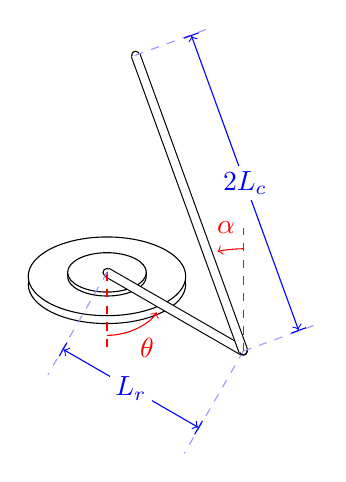
\begin{tikzpicture}
    \def\thetaone{60}
    \def\Lone{20mm}
    \def\thetatwo{20}
    \def\Ltwo{40mm}

    \base
    \begin{scope}[rotate=-90]
        \link{\thetaone:\Lone}
        \angann[0.8]{\thetaone}{$\theta$}
        \lineann[-1.5]{\thetaone}{\Lone}{$L_r$}
        \begin{scope}[shift=(\thetaone:\Lone), rotate=\thetaone + 120]
            \link{\thetatwo:\Ltwo}
            \angann[1.3]{\thetatwo}{$\alpha$}
            \lineann[-1]{\thetatwo}{\Ltwo}{$2L_c$}
        \end{scope}
    \end{scope}
\end{tikzpicture}
